%!TEX root = slides.tex

\section[Session 2]{Session 2: Empirical methods with which to detect
environmental and phenotypic associations: single and multiple locus
methodologies}

\begin{frame}
\frametitle{Detecting and dealing with population structure}
\begin{block}{Why is this important?}
\begin{itemize}
	\item{Can lead to spurious associations if not accounted for}
	\item{Population structure can look like LD}
	\item{Substantial and varying LD present in genome-scale datasets}
	\item{Which markers to use to access structure? - all of them}
	\item{Leave-one-out testing?}
\end{itemize}
\end{block}
\tiny
\citet{Price:2006cd}
\end{frame}

\begin{frame}
\frametitle{Detecting and dealing with population structure}
\begin{block}{}
\centering
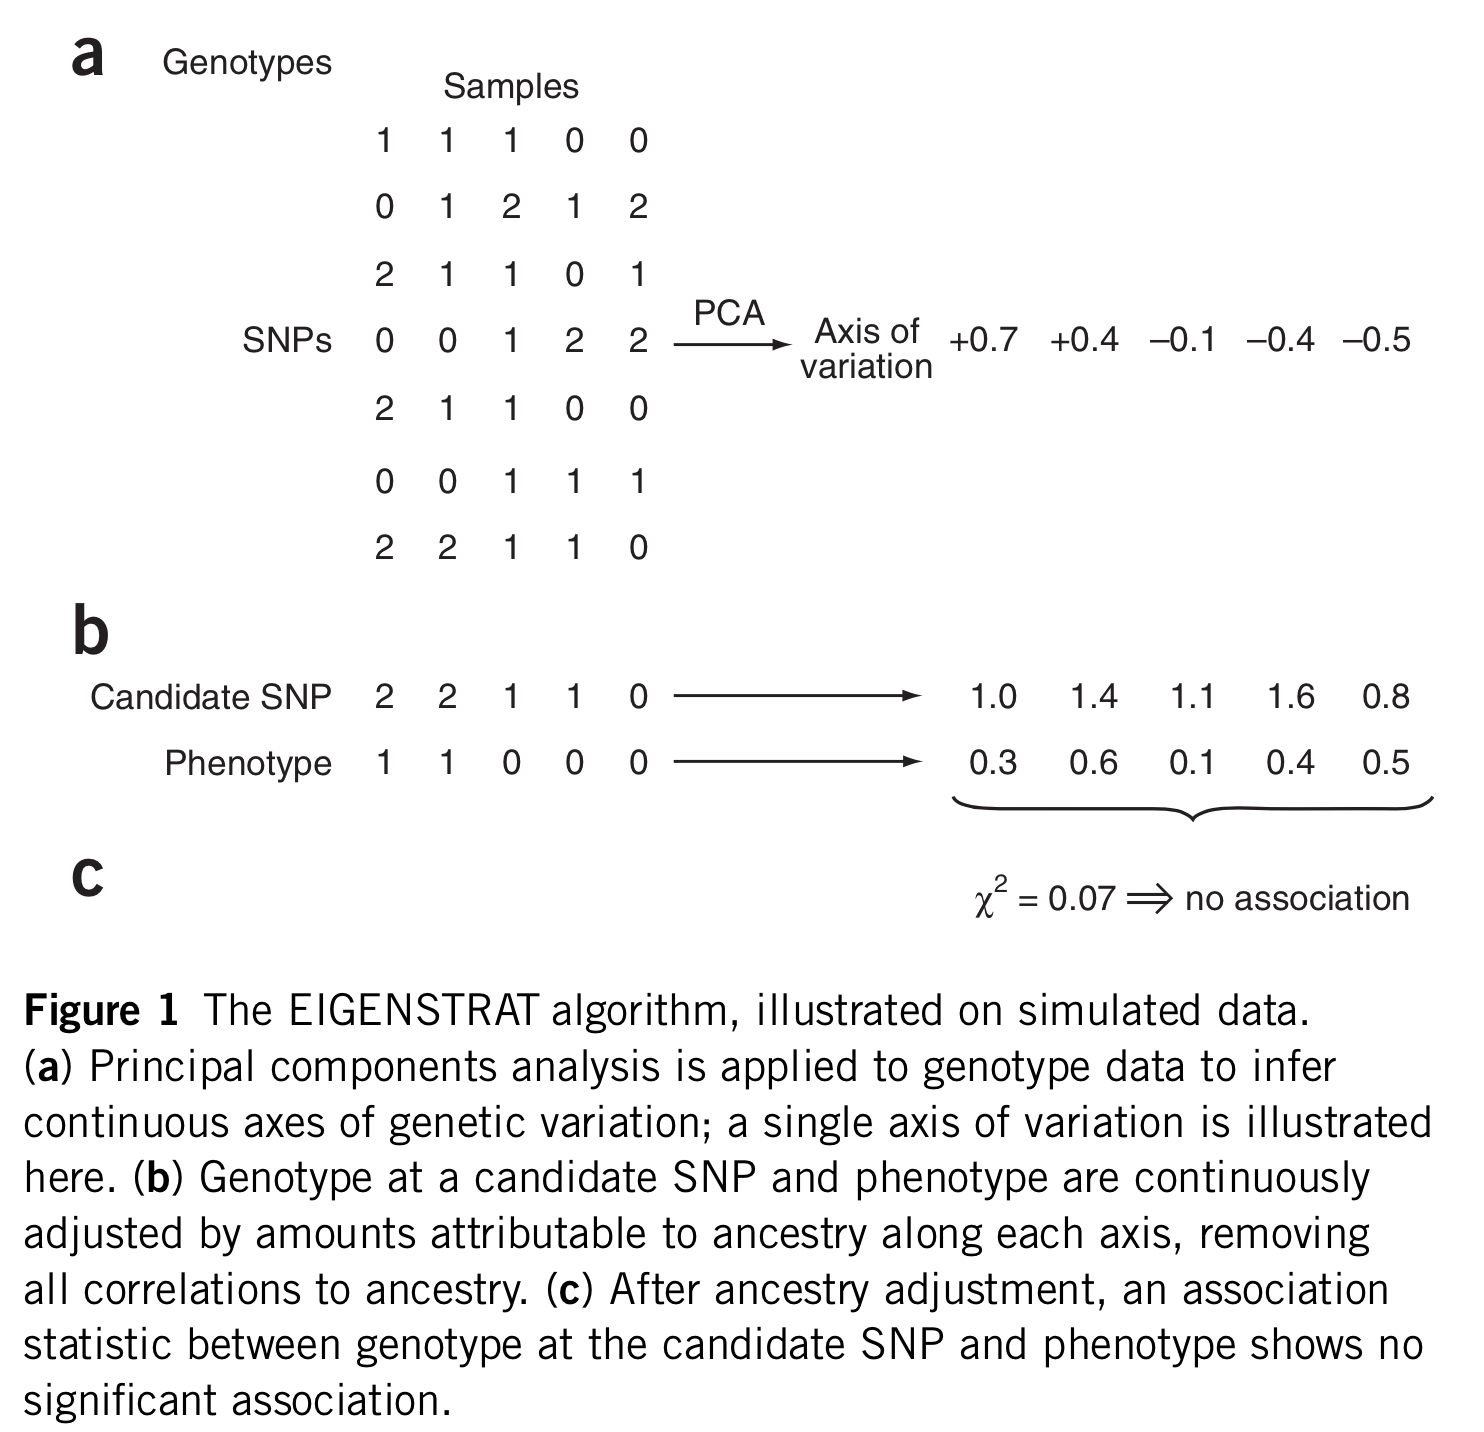
\includegraphics[height=0.8\textheight]{price.png}\\
\tiny
\citet[Figure 1]{Price:2006cd}
\end{block}
\end{frame}

\begin{frame}
\frametitle{Bayenv: identifying correlations with ecological variables}
\end{frame}